%%%%%%%%%%%%%%%%%%%%%%%%%%%%%%%%%%%%%%%%%
% University/School Laboratory Report
% LaTeX Template
% Version 3.1 (25/3/14)
%
% This template has been downloaded from:
% http://www.LaTeXTemplates.com
%
% Original author:
% Linux and Unix Users Group at Virginia Tech Wiki 
% (https://vtluug.org/wiki/Example_LaTeX_chem_lab_report)
%
% License:
% CC BY-NC-SA 3.0 (http://creativecommons.org/licenses/by-nc-sa/3.0/)
%
%%%%%%%%%%%%%%%%%%%%%%%%%%%%%%%%%%%%%%%%%

%----------------------------------------------------------------------------------------
%	PACKAGES AND DOCUMENT CONFIGURATIONS
%----------------------------------------------------------------------------------------

\newcommand{\abs}[1]{\left| #1 \right|} % for absolute value
\newcommand{\avg}[1]{\left< #1 \right>} % for average

\renewcommand{\d}[2]{\frac{d #1}{d #2}} % for derivatives
\newcommand{\dd}[2]{\frac{d^2 #1}{d #2^2}} % for double derivatives
\newcommand{\pd}[2]{\frac{\partial #1}{\partial #2}} 
% for partial derivatives
\newcommand{\pdd}[2]{\frac{\partial^2 #1}{\partial #2^2}} 
% for double partial derivatives
\newcommand{\pdc}[3]{\left( \frac{\partial #1}{\partial #2}
 \right)_{#3}} % for thermodynamic partial derivatives
\newcommand{\ket}[1]{\left| #1 \right>} % for Dirac bras
\newcommand{\bra}[1]{\left< #1 \right|} % for Dirac kets
\newcommand{\braket}[2]{\left< #1 \vphantom{#2} \right|
 \left. #2 \vphantom{#1} \right>} % for Dirac brackets
\newcommand{\matrixel}[3]{\left< #1 \vphantom{#2#3} \right|
 #2 \left| #3 \vphantom{#1#2} \right>} % for Dirac matrix elements
\newcommand{\grad}[1]{\gv{\nabla} #1} % for gradient
\let\divsymb=\div % rename builtin command \div to \divsymb
\renewcommand{\div}[1]{\gv{\nabla} \cdot #1} % for divergence
\newcommand{\curl}[1]{\gv{\nabla} \times #1} % for curl

\documentclass{article}

\usepackage{graphicx} % Required for the inclusion of images
\usepackage{natbib} % Required to change bibliography style to APA
\usepackage{amsmath}
\usepackage{setspace}
\usepackage{amssymb}
\usepackage{rotating}
\renewcommand{\labelenumi}{(\alph{enumi})}

%\setlength\parindent{0pt} % Removes all indentation from paragraphs

\renewcommand{\labelenumi}{\alph{enumi}.} % Make numbering in the enumerate environment by letter rather than number (e.g. section 6)

%\usepackage{times} % Uncomment to use the Times New Roman font

%----------------------------------------------------------------------------------------
%	DOCUMENT INFORMATION
%----------------------------------------------------------------------------------------

\title{WiPAL Fabry-P\'{e}rot\\ Spectrometer} % Title

\author{Ken \textsc{Flanagan} and Jason \textsc{Milhone}} % Author name

\date{\today} % Date for the report

\begin{document}

\maketitle % Insert the title, author and date


% If you wish to include an abstract, uncomment the lines below
% \begin{abstract}
% Abstract text
% \end{abstract}

%----------------------------------------------------------------------------------------
%	SECTION 1
%----------------------------------------------------------------------------------------

\section*{Introduction}

The Fabry-P\'{e}rot system on WiPAL is essentailly a very high-resolution spectrometer that can image the light emitted by ions in the plasma. This light will be doppler shifted by random movements of the ions (temperature) and by bulk ion flow. As a result, the spectrum captured represents the entire ion velocity distribution function (IVDF) . A reliable measurement of ion temperature and flow is essential for many WiPAL experiements,  such as dynamo stirring and MRI flow drive.

This brief write-up should serve as a good primer for anyone interested in using the WiPAL system as well as a good resource for those who may be building off of the work done to date.  In the first section, the optical layout of the system is described as it is currently used on WiPAL. Next, an overview of Fabry-P\'{e}rot theory is given to layout basic concepts. Next, using the basic Fabry-P\'{e}rot theory, a more detailed description within the context of spectrometry. Finally, the processes used in the analysis of Fabry-P\'{e}rot output are outlined along with a overview of the code used at WiPAL.

%----------------------------------------------------------------------------------------
%	SECTION 2
%----------------------------------------------------------------------------------------

\section{Basic Fabry-P\'{e}rot Theory}
A Fabry-P\'{e}rot interferometer consists of a set of highly-reflective, partially transmitting parallel plates, called an \'{e}talon. Light enters the \'{e}talon and is reflected many times back and forth creating an interference pattern. This pattern can be used to determine the wavelength of the incident light. 
\begin{figure}
\begin{center}
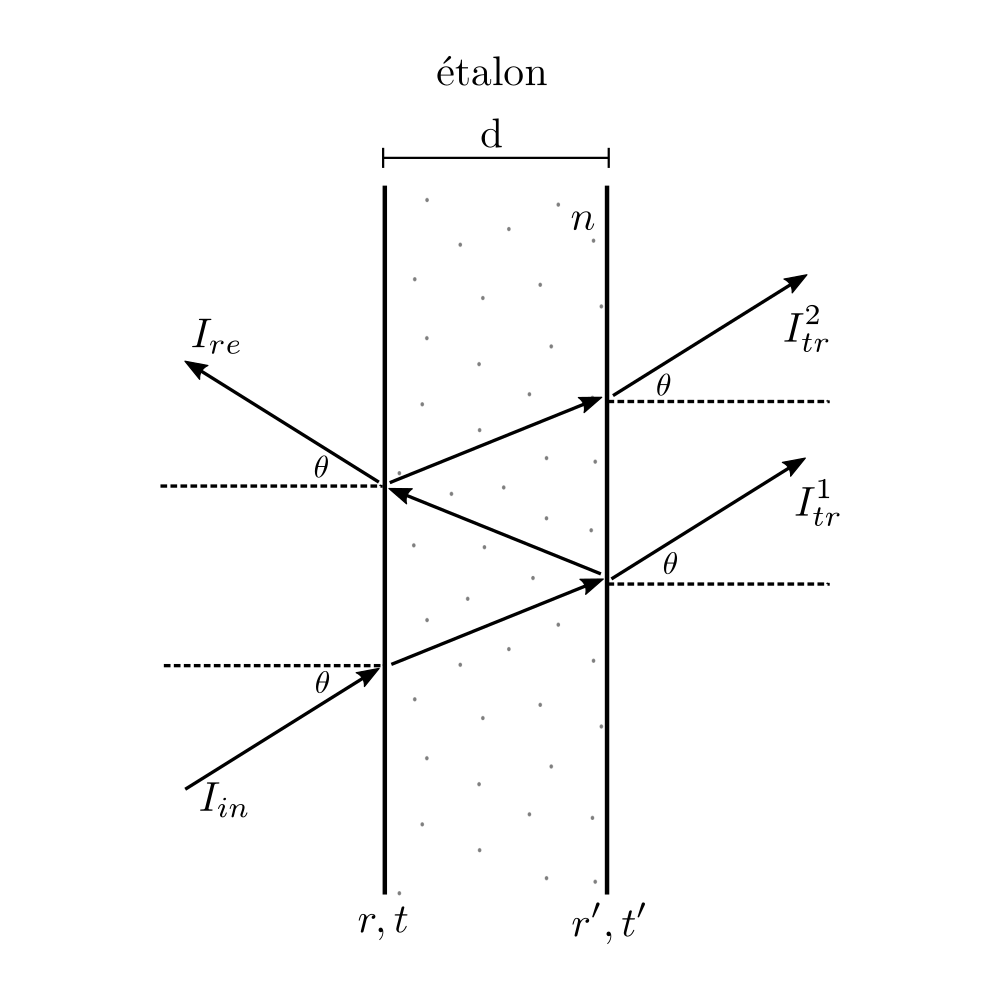
\includegraphics[scale=1]{Images/etalon.png}
\caption{An \'{e}talon showing incident, reflected and transmitted light.
\label{fig:etalon}}
\end{center}
\end{figure}
Fig.~\ref{fig:etalon} shows a simple schematic of an \'{e}talon. Light incident at some angle, $\theta$, reflects back and forth in the cavity and then exits at the same angle, $\theta$. The optical path difference between two beams exiting the \'{e}talon is
\begin{equation}
l_{opt} = 2nd\cos{\theta}
\end{equation}
where $n$ is the index of refraction in the \'{e}talon gap and $d$ is the width of the gap. We can calculate the phase shift between consective passes in the \'{e}talon by multiplying the wavenumber, $2\pi/\lambda$, by this optical path difference. 
\begin{equation}
\delta = \frac{2\pi}{\lambda}l_{opt}=2\pi \frac{2nd}{\lambda}\cos{\theta}=2\pi m
\label{eq:ph}
\end{equation}
where we have defined $m$ as the interference order number. When the phase difference is integer multiples of $2\pi$, we expect constructive interference to occur, thus the interference condition for a Fabry-P\'{e}rot \'{e}talon is
\begin{equation}
m=\frac{2nd}{\lambda}\cos{\theta}
\label{eq:int_con}
\end{equation}
Now we can work out the interference pattern by calculating the transmitted amplitude, $a_{tr}$ of incident light, $a_{in}$. Because we are working in amplitude, we will use amplitude reflectivities and transmissivities for the plates: $r$, $r'$ and $t$, $t'$, repectively. The square modulus of these reflectivities and transmissivities are the reflection and transmission coefficients of the \'{e}talon plates: $R$, $R'$ and $T$, $T'$, respectively. Summing up every beam in the \'{e}talon, we get a transmission amplitude of
\begin{align*}
a_{tr}&=tt'a_{in}+tt'a_{in}rr'e^{i\delta}+tt'a_{in}(rr')^{2}e^{2i\delta}+tt'a_{in}(rr')^{3}e^{3i\delta}+...\\
&=tt'a_{in}\sum_{p=0}^{\infty}(rr'e^{i\delta})^{p}=a_{in}\frac{tt'}{1-rr'e^{i\delta}}
\end{align*}
Now we need to take the square modulus of this ampltiude in order to get the transmitted intensity. This gives us
\begin{equation}
\frac{I_{tr}}{I_{in}}=\left|\frac{a_{tr}}{a_{in}}\right|^{2}=\frac{TT'}{\big|1-\sqrt{RR'}e^{i\delta}\big|^{2}}
\end{equation}
In order to clean up this expression some, we can introduce the coefficient
\begin{equation}
Q=\frac{4\sqrt{RR'}}{(1-\sqrt{RR'})^{2}}
\end{equation}
which leads us to
\begin{equation}
\frac{I_{tr}}{I_{in}}=\frac{TT'}{(1-\sqrt{RR'})^{2}}\left[1+Q\sin^{2}{\left(\frac{\delta}{2}\right)}\right]^{-1}
\end{equation}
which is recognizable as the Airy function. If the \'{e}talon plates have identical reflection and transmission coefficients, then the prefactor becomes unity. Also, we can replace the phase shift, $\delta$, with $2\pi m$ from eq.~\ref{eq:ph}. This gives us a transmission function of
\begin{equation}
\frac{I_{tr}}{I_{in}}=[1+Q\sin^{2}{(\pi m)}]^{-1}
\label{eq:airy}
\end{equation}
At interger $m$, this function has a maximum value of 1, showing us the interference condition that we found before in eq.~\ref{eq:int_con}. As seen if fig.~\ref{fig:airy} the FWHM of the transmission is dependent on $Q$. A higher $Q$ leads to narrower peaks, which means a higher resolving power of the \'{e}talon. Following convention, this $Q$ is sometimes replaced with a figure of merit of the \'{e}talon plates known as the finesse, $\mathcal{F}$, which is 
\begin{equation}
\mathcal{F}=\frac{\pi}{2}\sqrt{Q}
\end{equation}
The distance between successive peaks (which is one order number) is known as the free spectral range, FSR. Using the finesse, the FWHM of the Airy function is simply $FSR/\mathcal{F}$. 
\begin{figure}
\begin{center}
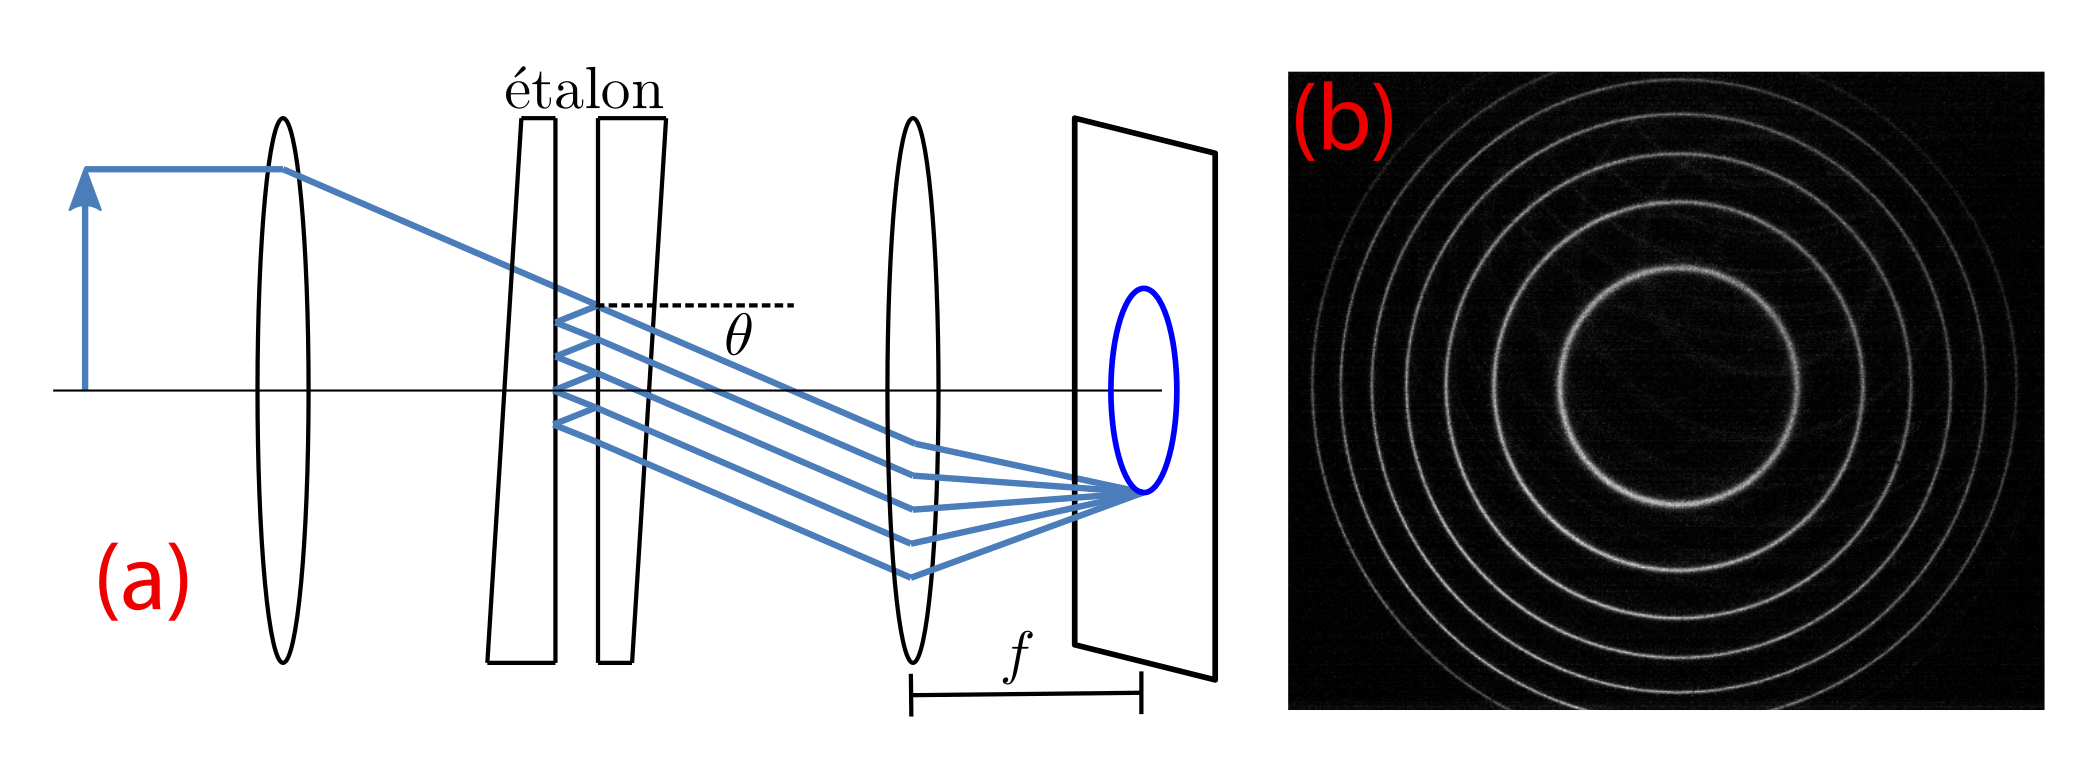
\includegraphics[width=\textwidth]{Images/ring_pattern.png}
\caption{A) diagram showning the focusing of the \'{e}talon ring pattern onto an imaging plane. B) Actually ring pattern recorded with the WiPAL Fabry-P\'{e}rot system.
\label{fig:real_rings}}
\end{center}
\end{figure}
\subsection*{Imaging Fabry-P\'{e}rot Rings}
If we plug in the expression for $m$ (eq.~\ref{eq:int_con}) into eq.~\ref{eq:airy} we get
\begin{equation}
\frac{I_{tr}}{I_{in}}=\left[1+Q\sin^{2}{\left(\frac{2nd}{\lambda}\cos{\theta}\right)}\right]^{-1}
\end{equation}
If $n$, $d$, and $\lambda$ are fixed, then the interference pattern will be peaks at ever increasing $\cos{\theta}$. This leads to the familiar ring pattern of the Fabry-P\'{e}rot. Now if we place a lens with focal length, $f$,  behind the \'{e}talon, we can focus this pattern on a plane. Defining $r$ as the radius on this plane (with the optical axis being the origin), 
\begin{equation}
\cos{\theta}=\frac{f}{\sqrt{f^{2}+r^{2}}}=\left[1+\left(\frac{r}{f}\right)^{2}\right]^{-1/2}
\end{equation}
Now we see that the Airy function can be written as a function in $r$ with $f$, $n$, $d$ and $\lambda$ fixed. 
\begin{equation}
\frac{I_{tr}}{I_{in}}=\left[1+Q\sin^{2}{\left(\frac{A}{\sqrt{1+(r/f)^{2}}}\right)}\right]^{-1}
\end{equation}
with $A=2\pi n d / \lambda$.  With this function the distance between interference peaks drops as we move out in $r$. This function is imaged in fig.~\ref{fig:real_rings}.

%----------------------------------------------------------------------------------------
%	SECTION 3
%----------------------------------------------------------------------------------------

\section{Fabry-P\'{e}rot Spectroscopy}
Fabry-P\'{e}rot spectroscopy maps the ring pattern output of the \'{e}talon to a source's spectrum by varying one or more of the variables in the interference condition (eq.~\ref{eq:int_con}). Traditionally, this is done by varying the index of refraction, $n$, by putting the \'{e}talon in a controllable pressure chamber. Alternatively, some \'{e}talons are outfized with a pizeoelectric driver that can very slight change the distance between the plates, $d$. 	At WiPAL, however, we do not have time during a plasma discharge to vary these parameters, so we rely on calibration to a known wavelength and compare ring locations and widths to map out the plasma spectrum.

Calibration is performed using a hollow-cathode Thorium lamp. Thorium is a great calibration source because it is a very heavy atom that has no isotopes (therefore, the line broadening is extremely small). In order to get a $m$, $d$ and $f$, the peak locations of the thorium rings are found and successive orders are used to solve the interference condition based on these locations using the NIST database thorium wavelength. 

\subsection*{Ring Locations}
Given the interference condition (eq.~\ref{eq:int_con}) and the Airy function output of the interferometer (eq.~\ref{eq:airy}), the output of the Fabry-P\'{e}rot for a given wavelength can be calculated. Looking at the interference condition, $m$ for a given $\lambda$ is given by 
\begin{equation}
m = 0,\,1,\,2\,...\,m_{0}\leq\frac{2d}{\lambda}
\end{equation}
where $m_{0}$ must be less than the $m$ given on the optical axis (when $\cos{\theta}=1$), $2d/\lambda$. Written another way,
\begin{equation}
m_{0} = \text{m of first interference peak} = \frac{2d}{\lambda} - \epsilon
\end{equation}
where $0\leq\epsilon<1$. Or, even simpler, $m_{0}=\text{Floor}[2d/\lambda]$. The interference condition is met by integer $m$, so this means that subsequent peaks will have $m_{j}=m_{0}-j$ for $j=0,\,1,\,2\,...$. (Note: $m$ decreases as we move away from the optical axis, because $\cos{\theta}$ decreases from $\theta=0$ to $\theta=\pi/2$.) In terms of the interference condition, this gives us:
\begin{equation}
m_{j}=m_{0}-j =\frac{2d}{\lambda}\frac{f}{\sqrt{f^{2}+r_{j}^{2}}}
\label{eq:mj}
\end{equation}
where $r_{j}$ is the radial location of peaks for that given wavelength. Inverting this equation to solve for peak locations gives,
\begin{equation}
r_{j} = f\sqrt{\left(\frac{2d/\lambda}{m_{0}-j}\right)^{2}-1}=f\sqrt{\left(\frac{2d/\lambda}{\text{Floor}[2d/\lambda]-j}\right)^{2}-1}
\end{equation}


All of the above calculation works for a given, single wavelength, but we are interested in what the Fabry-P\'{e}rot output for a given input spectrum, $B(\lambda)$, looks like. For this we need to integrate over all wavelengths. The output as a function of radius across the ccd will be:
\begin{equation}
I(r) = \int_{0}^{\infty} \frac{B(\lambda)\,d\lambda}{1+Q\sin^{2}{\left(\pi \frac{2d}{\lambda}\frac{f}{\sqrt{f^{2}+r^{2}}}\right)}}
\label{eq:pattern}
\end{equation}

\subsection*{Mapping $r$ to $\lambda$}
In order to extract spectral information from the interference pattern given by eq.~\ref{eq:pattern}, a mapping must be made from $r$ to $\lambda$ space. This can be done by considering the change in $r$, $\Delta r$, for a given change in $\lambda$, $\Delta\lambda$. From eq.~\ref{eq:mj}, we see that if $\lambda\rightarrow\lambda+\Delta\lambda$, $r_{j}\rightarrow r_{j}+\Delta r$ in order to keep $m_{j}$ an integer. If we limit the change in $\lambda$ to less than a free spectral range, then
\begin{equation}
m_{0}=\text{Floor}\left[\frac{2d}{\lambda_{0}}\right]=\text{Floor}\left[\frac{2d}{\lambda_{0}+\Delta\lambda}\right]
\end{equation}
Under this condition we have a relation between $\Delta\lambda$ and $\Delta r$ given by
\begin{equation}
m_{0}-j = \frac{2d}{\lambda_{0}+\Delta\lambda}\frac{f}{\sqrt{f^{2}+(r_{j}-\Delta r)^{2}}}
\end{equation}
Solving for $\Delta r$, we get
\begin{equation}
\Delta r = r_{j} \pm f \sqrt{\left(\frac{2d}{(m_{0}-j)(\lambda_{0}+\Delta\lambda)}\right)^{2}-1}
\label{eq:dr1}
\end{equation}
This relation works quite well if you know $\lambda_{0}$, as is the case for a calibration lamp or a non-flowing plasma. However, if $\lambda_{0}$ isn't well known (only within a free spectral range-- which corresponds to a flow velocity of about 60 km/s for the Argon 488nm line), we can use eq.~\ref{eq:mj} to get $\lambda_{0}$ given $r_{j}$.
\begin{equation}
\lambda_{0}=\frac{2d}{m_{0}-j}\frac{f}{\sqrt{f^{2}+r_{j}^{2}}}
\label{eq:lam_sub}
\end{equation}
Now if we substitute this into eq.~\ref{eq:dr1}, we have
\begin{equation}
\Delta r = r_{j} \pm f\sqrt{\left(\frac{2d\sqrt{f^{2}+r_{j}^{2}}}{2df+\Delta\lambda(m_{0}-j)\sqrt{f^{2}+r_{j}^{2}}}\right)^{2}-1}
\label{eq:dr2}
\end{equation}
Now we need to satisfy our condition that we don't venture out of a free spectral range when doing this mapping. To start, we should figure out what $\Delta\lambda$ gives the same $r$ location for two consecutive orders. Because increasing $r$ means decreasing $\lambda$ and orders decrease as $r$ is decreased we have:
\begin{align}
m_{0}-j&=\frac{2d}{\lambda_{0}-\Delta\lambda}\frac{f}{\sqrt{f^{2}+r_{edge}^{2}}}\\
m_{0}-j-1&=\frac{2d}{\lambda_{0}+\Delta\lambda}\frac{f}{\sqrt{f^{2}+r_{edge}^{2}}}
\end{align}
solving for $r_{edge}$ in both these equations and setting the resulting expressions equal gives
\begin{equation}
\Delta\lambda_{FSR/2}=\frac{\lambda_{0}}{2(m_{0}-j)-1}=\frac{2d}{2(m_{0}-j)^{2}-(m_{0}-j)}\frac{f}{\sqrt{f^{2}+r_{j}^{2}}}
\end{equation}
where we have used eq.~\ref{eq:lam_sub} to substitute $\lambda_{0}$ with an expression using $r_{j}$. Now we can take this expression and plug it into eq.~\ref{eq:dr2} to get the range of $r$ for a given order. 




\section{Line Shape Math}

\subsection{Doppler Broadened Shifted Maxwellian}

\begin{equation}
f = f_0 ( 1 + \frac{V+v}{c} )
\end{equation}

\begin{equation}
\frac{\Delta \lambda}{\lambda} = - \frac{\Delta f}{f}
\end{equation}

\begin{equation}
v = c (1 - \frac{\lambda}{\lambda_0}) - V
\end{equation}

\begin{equation}
P_v(v) dv = P_{\lambda} d \lambda = P_v ( v(\lambda) ) \frac{c}{\lambda_0} d\lambda
\end{equation}

\begin{equation}
P_v(v) dv = \sqrt{\frac{m}{2 \pi k_B T}} e^{- \frac{m v^2}{2 k_B T}}
\end{equation}

\begin{equation}
P_{\lambda}(\lambda) d \lambda = \sqrt{\frac{m c^2}{2 \pi k_B T \lambda^2}} e^{-\frac{m}{2 k_B T} \left(c(1-\lambda / \lambda_0 ) - V \right)^2}
\end{equation}

\begin{equation}
P_{\lambda}(\lambda) d \lambda = \frac{1}{\sqrt{2 \pi} \sigma} e^{-\frac{\left(\lambda - \lambda_0(1 - V/c)\right)^2}{2 \sigma^2}}
\end{equation}

\begin{equation}
\sigma = \sqrt{\frac{k_B T}{m}} \frac{\lambda_0}{c} = \frac{V_{th}}{c} \lambda_0
\end{equation}

\subsection{Instrument Function and Doppler Broadening}

Instrument function is a Lorentzian

\begin{equation}
L(x;\mu,\gamma) = \frac{\gamma / \pi}{(x-\mu)^2 + \gamma^2}
\end{equation}

where $\mu$ is the center, and $\gamma$ is the half-width at half-maximum.  The doppler broadened line shape is given by a gaussian.

\begin{equation}
G(x;\mu, \sigma) = \frac{1}{\sigma \sqrt{2 \pi}} e^{-(x-\mu)^2 / 2 \sigma^2}
\end{equation}

The line profile imaged by the CCD in $\lambda$-space is given by

\begin{equation}
V(x;\mu,\sigma,\gamma) = \int_{-\infty}^{\infty} G(x';\mu,\sigma) L(x-x';\mu,\gamma) dx' 
\end{equation}

This can be rewritten in terms of the complex Faddeeva function, $w(z)$.

\begin{equation}
 V(x;\mu,\sigma,\gamma) = \frac{\rm{Re}[w(z)]}{\sigma \sqrt{2 \pi}} \quad z=\frac{x - \mu + i \gamma}{\sigma \sqrt{2}}
\end{equation} 
%----------------------------------------------------------------------------------------
%	SECTION 4
%----------------------------------------------------------------------------------------

\section{Optical Layout}
\begin{figure}
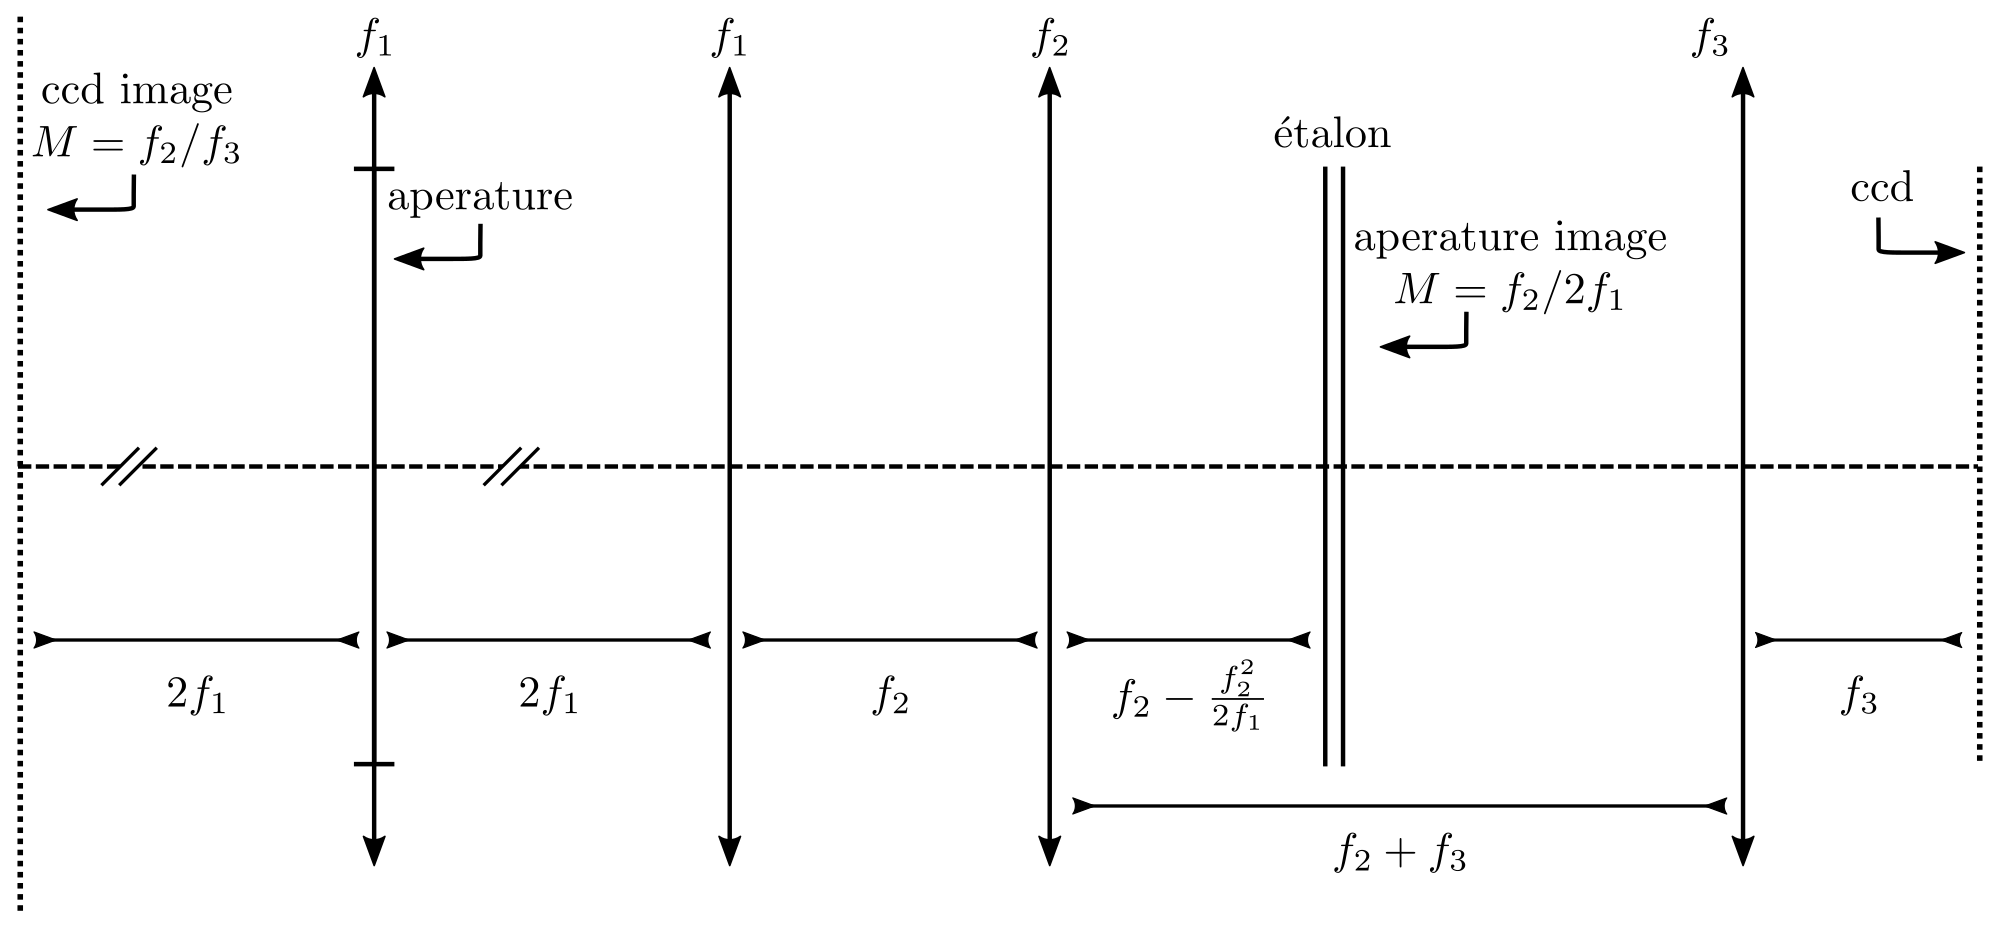
\includegraphics[width=\textwidth]{Images/OpticalLayout.png}
\caption{Optical schematic of Fabry-P\'{e}rot spectrometer used on WiPAL. All lengths are in units of millimeters. \label{fig:opticalsetup}}
\end{figure}
The optical layout for the WiPAL Fabry-P\'{e}rot spectrometer is shown above in Fig.~\ref{fig:opticalsetup}. The main components of this setup are a pair of lenses of focal length, $f_{1}$, that form a telescope to bring light from the center of plasma to the \'{e}talon, another telescope formed by lenses $f_{2}$ and $f_{3}$ that focuses light through the \'{e}talon, and the camera sensor.

The telescope formed by the $f_{1}$ lenses acts to extend the image plane of the sensor a distance $2f_{1}$ past the first lens. For WiPAL, we have chosen $f_{1}=1000$ mm, so the ccd image plane is 2m past the first lens of the system, which is roughly the center of the plasma. The lenses with focal length $f_{2}$ and $f_{3}$ function to magnify the ccd image by a factor of $f_{2}/f_{3}$. So for a sensor that is $\sim15$ mm and lenses $f_{2}=350$ mm and $f_{3}=150$ mm, the image of the ccd in the plasma is roughly 35 mm. This area of the image in the focus plane is essentially the beam diameter of the chord of light sampled by the spectrometer.

An aperature is placed at the first lens of the system in order to control the illuminated spot size on the etalon. Imaging this aperature through the system places it's image $f_{2}-f_{2}^{2}/2f_{1}$  past the $f_{2}$ lens with a magnification of $f_{2}/2f_{1}$. If $f_{2}<f_{1}$, which is the case for the WiPAL system, the aperature image will be smaller than the actual aperature. It is important to use a small spot size on the \'{e}talon in order to minimize the effect of plate defects over the surface.

For the WiPAL system, table~\ref{tab:system} lists the values of optical components used. These values have been chosen to optimize the imaging of the interference pattern of the \'{e}talon and to maximize the amount of light collected from the plasma. 
\begin{table}
\begin{center}
\begin{tabular}{l | l }
parameter & value \\\hline
$f_{1}$ & 1000 mm\\
$f_{2}$ & 350 mm\\
$f_{3}$ & 150 mm\\
$M_{ccd}$ & 7/3 \\
$M_{aperature}$ & 0.175\\
ccd & 15.6 mm\\
beam size & 36.4 mm\\
aperature & 40 mm\\
spot size & 7 mm
\end{tabular}
\caption{A table of chosen values for optical components of the WiPAL Fabry-P\'{e}rot system.}
\label{tab:system}
\end{center}
\end{table}

%----------------------------------------------------------------------------------------
%	BIBLIOGRAPHY
%----------------------------------------------------------------------------------------

%\bibliographystyle{apalike}

%\bibliography{sample}

%----------------------------------------------------------------------------------------


\end{document}
